\documentclass{article}
\usepackage[utf8]{inputenc}

\usepackage{natbib}
\usepackage{graphicx}
\usepackage{fancyhdr}
\usepackage{amsthm}

\theoremstyle{definition}
\newtheorem{definition}{Definition}[section]

\pagestyle{fancy}
\fancyhf{}
\fancyfoot[L]{Unless otherwise specififed, all content is the author's summary of "Goodfellow, Ian, Yoshua Bengio, and Aaron Courville. Deep learning. MIT press, 2016." with some text verbatim. For the full text, please visit: http://www.deeplearningbook.org/.}

\title{Deep Learning Textbook - Notes}
\author{yusuf.roohani }
\date{Began August 2017}

\begin{document}
\maketitle

%%% ---- SECTION 1 Prboability

\section{Probability}

\subsection{Distributions}

\begin{itemize}
    \item Probability mass functions:\\
    State of the random variable $\mapsto$ Probability of the variable taking on that state
    
    \item Joint probability functions:
    Probability distribution over multiple variables
    
    \item 
    For any probability mass function:
    \begin{itemize}
    \item Domain of P should be all possible states of x
    \item $\forall$ $x \in$ x, $ 0 \leq P(x) < 1$
    \item $\sum_{x \in \textrm{x}} P(x) = 1$
    \end{itemize}
\end{itemize}

%%% ---- SECTION 4 Numerical Computations

\section{Numerical Computations}

\begin{definition}{Numerical computation}
Algorithms that solve mathematical problems by methods that update estimates of the solution via an iterative process, rather than analytically deriving a formula
\end{definition}

Fundamental difficulty with digital computers - infinitely many real numbers need to be represented with a finite number of patterns. Thus there is necessarily some approximation.

\subsection{Overflow and Underflow}

\begin{definition}{Underflow}
When numbers near zero are rounded to zero
\end{definition}

\begin{definition}{Overflow}
When numbers with large magnitude are approximated as $\infty$ or $-\infty$
\end{definition}

For instance, in the softmax function

$$ \textrm{softmax}(x)_i = \frac{exp(x_i)}{\sum^n_{j=1}exp(x_j)} $$

Assume all $x_i$ are equal to $c$. If $c$ is too large, there will be underflow and the final result is undefined. If $c$ is very large and positive $exp(c)$ will overflow and it will also be undefined. One solution is to calculate the softmax as

$$ \textrm{softmax}(z) = x - max_ix_i $$

These are just some examples of numerical issues that are generally handled by low level libraries.

\subsection{Gradient based optimization}

\begin{definition}{Optimization}
Either minimizing or maximizing some (objective or cost) function $f(x)$ by altering $x$. Optimum value usually denoted as $x^*$
\end{definition}

The derivative $f'(x)$ gives the slope of $f(x)$ at the point x.

$$ f(x + \epsilon) \approx f(x) + \epsilon f'(x) $$

\begin{definition}{Gradient descent}
Reduce f(x) by moving in small steps with the opposite sign of the derivative
\end{definition}

A local minimum is a point where $f(x)$ is lower than at all neighboring points. A global minimum is the absolute lowest value of $f(x)$

In the context of deep learning, we optimize functions that may have many local minima that are not optimal and many saddle points surrounded by very flat regions. All of this make optimization difficult especially for multimdimensional functions.

We must now generalize to multiple dimensions.

\begin{definition}{Gradient}
The gradient is the vector containing all the partial derivatives. Element $i$ of the gradient $ \nabla_xf(x)$ is the partial derivatives of $f$ with respect to $x_i$. 
\end{definition}

\begin{definition}{directional derivative}
The directional derivative in $u$ (unit vector) is the slope of the function $f$ in direction $u$

$$ \frac{\partial}{\partial a} f(x + au) = u^T\nabla_xf(x) $$
\end{definition}

Minimizing this equation:
$$ \min_{u, u^Tu=1} u^T\nabla_xf(x) $$
$$ \min_{u, u^Tu=1} ||u||_2 ||\nabla_xf(x)||_2 cos\theta $$

This will be minimized in the direction opposite to the gradient $(cos \theta = -1)$ We can thus decrease $f$ by moving in the direction of the negative gradient.

$$ x' = x - \epsilon\nabla_xf(x) $$

Here $\epsilon$ is the learning rate, a scalar that determines the size of the step.

\subsection{Jacobian and Hessian Matrices}

%%% ---- SECTION 5 Machine Learning

\section{Machine Learning}

\begin{definition}
Machine learning is a branch of applied statistics with increased emphasis on the use of computer to estimtate complicated functions
\end{definition}

\begin{definition}
{Learning} A computer program is said to learn from experience $E$ with respect to some class of tests $T$ and performance measure $P$, if its performance at tasks in $T$, as measured by $P$ improves with experience $E$
\end{definition}

Tasks are usually defined in terms of how a machine learning algorithm should process an example. An example is a collection of features that have been quantitatively measured from some object.

Some common machine learning tasks:
\begin{itemize}
    \item Classification
    \item Classification with missing inputs
    \item Regression
    \item Transcription
    \item Machine translation
    \item Structured output
    \item Anomaly detection
    \item Synthesis and sampling
    \item Imputation of missing values
    \item Denoising
    \item Density estimation
\end{itemize}

The performance measure is a quantitative measure of performance, eg: accuracy, error rate.

Machine learning algorithms are generally allowed to experience an entire dataset.
\begin{definition}
{Unsupervised learning} Learn the entire probability distirubtion that generated a dataset, whether explicitly, as in density estimation, or implicitly, such as in synthesis and denoising
\end{definition}

\begin{definition}
{Supervised learning} Experience a dataset where each example is associated with a label.
\end{definition}

\subsection{Capacity, Overfitting, Underfitting}

Central challenge in machine learning: model must perform well on new, unseen inputs (generalization). The generalization error is the expected value of the error for a new input.

What separates machine learning from optimization is that we want generalization error to be low as well as training error. This is normally estimated through performance on a test set.

How can we affect performance on test set when we only see the training set

We typically make a set of assumptions (i.i.d. assumptions):
\begin{itemize}
    \item Examples in each dataset (train or test) are independent of each other
    \item training and test set are identically distributed (i.e. same data generating distribution)
\end{itemize}

Thus, for a randomly selected model, the expected training error is equal to the expected test error. However, in machine learning, we sample the training set, use it to choose parameters to reduce the training set error, then sample the test set. Now, expected test error is greater than training

So we must 
\begin{itemize}
    \item Make the test error small (to prevent underfitting)
    \item Reduce the gap between training and test (to prevent overfitting)
\end{itemize}

Both of these can be altered using model capacity. Eg: with high capacity you learn unimportant properties from training set

\section{Neural Networks}

\begin{itemize}
    \item \textbf{Softmax} The softmax function is normally used to highlight the largest values and suppress values which are significantly below the maximum value
\end{itemize}

\section{Regularization}
Central problem in machine elarning is to perform well not only on training data, but also on new inputs. \textbf{Regularization refers to any modification to a learning algorithm that is intended to reduce its generalization error but not its training error}

In deep learning, a common approach is to regularize estimators: this is done by trading increased bias for reduced variance. Try to improve effectiveness by making a profitable trade. Models are generally in three regimes
\begin{itemize}
    \item \textbf{Underfitting}: Exclude the true data-generating process
    \item Matched the true data generating process
    \item \textbf{Overfitting}: Include the process but also many other possible generating processes
\end{itemize}
The goal of regularization is to take a model from the third regime to the second regime. What we generally find is that the best fitting model is a large model that has been regularized appropriately.

\subsection{Parameter Norm Penalties}

Limit the capacity of models by adding a paramter norm penalty $\Omega(\theta)$ to the objective function $J$. 
$$ \tilde{J}(\theta; X, y) = J( \theta; X, y) + \alpha\Omega(\theta) $$

where $ \alpha \in [0, \infty) $ is a hyperparamter that weighs the relative contribution of the norm penalty term, $\Omega$, relative to the standard objective function J.

So the training algorithm will decrease both $J$ and some measure of the size of some subset of the parameters $ \theta$.

Generally, for neural networks, we \textbf{only penalize the weights of the affine transformation and not the biases}. Bias controls only a single variable whereas the weights determine how two variables interact. Regularizing bias can induce significant underfitting.

\begin{itemize}
    \item \textbf{$L^2$ Regularization} Also known as the weight decay, this regularization strategy drives the weights closer to the origin by adding a term $ \Omega(\theta) = \frac{1}{2} || w ||^2_2$
    
    So, the objective function can be written as:
    $$ \tilde{J}(w; X, y) = J(w; X, y) + \frac{\alpha}{2}w^Tw $$
    
    And the update step after simplification becomes:
    $$ w \leftarrow (1 - \epsilon\alpha)w - \epsilon \nabla_wJ(w; X,y) $$
    
    Clearly, there is a multiplicative shrinking of the weight vector by a constant factor on each step.
    
    ----
    
    Only directins along which the paramters contribute significantly to reducing the objective function are preserved relatively intact. In others, a small Eigen value of the Hessian tells us that movement in that direction will not significantly increase the gradient.
    
    In the specific case of linear regression, this equation is simplified to:
    $$ w = (X^TX + \alpha I) ^{-1} X^T y $$
    
    Since the diagonal entries of $ (X^TX + \alpha I)$ correspond to the variance of each input feature, we see that $L^2$ regularization causes $X$ to appear as though it has higher variance. The algorithm thus shrinks weights on features whose covariance with the output target is low compared with the added variance .
    
    \item{$L^1$ Regularization} - Here we add the absolute value of the individual parameters to $J$
    
    $$ \Omega(\theta) = ||w||_1 = \sum_i|w_i| $$
    
\end{itemize}

\section{Optimization}

\section{Convolutional Neural Networks}

\section{Applications}


\begin{figure}[h!]
\centering
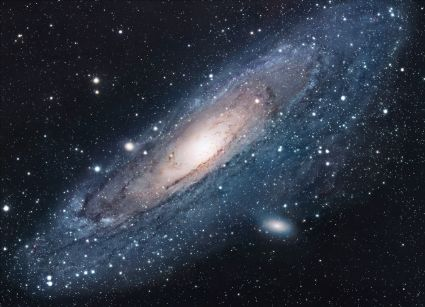
\includegraphics[scale=1.7]{universe.jpg}
\caption{The Universe}
\label{fig:univerise}
\end{figure}

\section{Conclusion}
``I always thought something was fundamentally wrong with the universe'' \citep{adams1995hitchhiker}

\bibliographystyle{plain}
\bibliography{references}

\end{document}
